        %%******************************************%%
        %%                                          %%
        %%        Modello di tesi di laurea         %%
        %%            di Andrea Giraldin            %%
        %%                                          %%
        %%             2 novembre 2012              %%
        %%                                          %%
        %%******************************************%%


% I seguenti commenti speciali impostano:
% 1. 
% 2. PDFLaTeX come motore di composizione;
% 3. tesi.tex come documento principale;
% 4. il controllo ortografico italiano per l'editor.

% !TEX encoding = UTF-8
% !TEX TS-program = pdflatex
% !TEX root = tesi.tex
% !TEX spellcheck = it-IT

\documentclass[10pt,                    % corpo del font principale
               a4paper,                 % carta A4
               twoside,                 % impagina per fronte-retro
               openright,               % inizio capitoli a destra
               english,                 
               italian,                 
               ]{book}    

\usepackage[utf8]{inputenc}             % codifica di input; anche [latin1] va bene
                                        % NOTA BENE! va accordata con le preferenze dell'editor

%**************************************************************
% Importazione package
%************************************************************** 

%\usepackage{amsmath,amssymb,amsthm}    % matematica

\usepackage[english, italian]{babel}    % per scrivere in italiano e in inglese;
                                        % l'ultima lingua (l'italiano) risulta predefinita

\usepackage{bookmark}                   % segnalibri

\usepackage{caption}                    % didascalie

\usepackage{chngpage,calc}              % centra il frontespizio

\usepackage{csquotes}                   % gestisce automaticamente i caratteri (")

\usepackage{emptypage}                  % pagine vuote senza testatina e piede di pagina

\usepackage{epigraph}					% per epigrafi

\usepackage{eurosym}                    % simbolo dell'euro

\usepackage[T1]{fontenc}                % codifica dei font:
                                        % NOTA BENE! richiede una distribuzione *completa* di LaTeX

%\usepackage{indentfirst}               % rientra il primo paragrafo di ogni sezione

\usepackage{graphicx}                   % immagini

\usepackage{hyperref}                   % collegamenti ipertestuali



\usepackage[binding=5mm]{layaureo}      % margini ottimizzati per l'A4; rilegatura di 5 mm

\usepackage{listings}                   % codici

\usepackage{microtype}                  % microtipografia

\usepackage{mparhack,fixltx2e,relsize}  % finezze tipografiche

\usepackage{nameref}                    % visualizza nome dei riferimenti                                      

\usepackage[font=small]{quoting}        % citazioni

\usepackage{subfig}                     % sottofigure, sottotabelle

\usepackage[italian]{varioref}          % riferimenti completi della pagina

\usepackage[dvipsnames]{xcolor}         % colori

\usepackage{booktabs}                   % tabelle                                       
\usepackage{tabularx}                   % tabelle di larghezza prefissata                                    
\usepackage{longtable}                  % tabelle su più pagine                                        
\usepackage{ltxtable}                   % tabelle su più pagine e adattabili in larghezza

\usepackage[toc, acronym]{glossaries}   % glossario
                                        % per includerlo nel documento bisogna:
                                        % 1. compilare una prima volta tesi.tex;
                                        % 2. eseguire: makeindex -s tesi.ist -t tesi.glg -o tesi.gls tesi.glo
                                        % 3. eseguire: makeindex -s tesi.ist -t tesi.alg -o tesi.acr tesi.acn
                                        % 4. compilare due volte tesi.tex.

\usepackage[backend=biber,style=verbose-ibid,hyperref,backref]{biblatex}
                                        % eccellente pacchetto per la bibliografia; 
                                        % produce uno stile di citazione autore-anno; 
                                        % lo stile "numeric-comp" produce riferimenti numerici
                                        % per includerlo nel documento bisogna:
                                        % 1. compilare una prima volta tesi.tex;
                                        % 2. eseguire: biber tesi
                                        % 3. compilare ancora tesi.tex.

%**************************************************************
% file contenente le impostazioni della tesi
%**************************************************************

%**************************************************************
% Frontespizio
%**************************************************************
\newcommand{\myName}{Luca De Franceschi}                                    % autore
\newcommand{\myTitle}{Sviluppo di un'applicazione Android per un sistema peer-to-peer di apprendimento di una lingua straniera}                    
\newcommand{\myDegree}{Tesi di laurea triennale}                % tipo di tesi
\newcommand{\myUni}{Università degli Studi di Padova}           % università
\newcommand{\myFaculty}{Corso di Laurea in Informatica}         % facoltà
\newcommand{\myDepartment}{Dipartimento di Matematica}          % dipartimento
\newcommand{\myProf}{Tullio Vardanega}                                % relatore
\newcommand{\myLocation}{Padova}                                % dove
\newcommand{\myAA}{2014-2015}                                   % anno accademico
\newcommand{\myTime}{Feb 2015}                                  % quando

\newcommand{\glossario}[1]{\textit{#1\ped{\ped{G}}}}            % per il glossario


%**************************************************************
% Impostazioni di impaginazione
% see: http://wwwcdf.pd.infn.it/AppuntiLinux/a2547.htm
%**************************************************************

\setlength{\parindent}{14pt}   % larghezza rientro della prima riga
\setlength{\parskip}{0pt}   % distanza tra i paragrafi


%**************************************************************
% Impostazioni di biblatex
%**************************************************************
\bibliography{bibliografia} % database di biblatex 

\defbibheading{bibliography}
{
    \cleardoublepage
    \phantomsection 
    \addcontentsline{toc}{chapter}{\bibname}
    \chapter*{\bibname\markboth{\bibname}{\bibname}}
}

\setlength\bibitemsep{1.5\itemsep} % spazio tra entry

\DeclareBibliographyCategory{opere}
\DeclareBibliographyCategory{web}

\addtocategory{opere}{womak:lean-thinking}
\addtocategory{web}{site:agile-manifesto}

\defbibheading{opere}{\section*{Riferimenti bibliografici}}
\defbibheading{web}{\section*{Siti Web consultati}}


%**************************************************************
% Impostazioni di caption
%**************************************************************
\captionsetup{
    tableposition=top,
    figureposition=bottom,
    font=small,
    format=hang,
    labelfont=bf
}

%**************************************************************
% Impostazioni di glossaries
%**************************************************************

%**************************************************************
% Acronimi
%**************************************************************
\renewcommand{\acronymname}{Acronimi e abbreviazioni}

\newacronym[description={\glslink{apig}{Application Program Interface}}]
    {api}{API}{Application Program Interface}

\newacronym[description={\glslink{cto}{Chief Technical Officer}}]
    {cto}{CTO}{Chief Technical Officer}

\newacronym[description={\glslink{cpo}{Chief Process Officer}}]
    {cpo}{CPO}{Chief Process Officer}

\newacronym[description={\glslink{ceo}{Chief Executive Officer}}]
    {ceo}{CEO}{Chief Executive Officer}

\newacronym[description={\glslink{html}{HyperText Markup Language}}]
    {html}{HTML}{HyperText Markup Language}

\newacronym[description={\glslink{rest}{Representational State Transfer}}]
    {rest}{REST}{Representational State Transfer}   

\newacronym[description={\glslink{DSL}{Domain Specific Language}}]
    {dsl}{DSL}{Domain Specific Language}  

\newacronym[description={\glslink{IDE}{Integrated Development Environment}}]
    {ide}{IDE}{Integrated Development Environment}  
   
%**************************************************************
% Glossario
%**************************************************************
\renewcommand{\glossaryname}{Glossario}

\newglossaryentry{refactoring}
{
    name=\glslink{refactoring}{refactoring},
    text=refactoring,
    sort=refactoring,
    description={In ingegneria del software, è una tecnica strutturata per modificare la struttura interna di porzioni di codice senza modificarne il comportamento esterno applicata per migliorare alcune caratteristiche non funzionali del software. I vantaggi che il refactoring persegue riguardano in genere un miglioramento della leggibilità, della manutenibilità, della riusabilità e dell'estendibilità del codice e la riduzione della sua complessità, eventualmente attraverso l'introduzione a posteriori di design pattern.}
}

\newglossaryentry{freeze}
{
    name=\glslink{freeze}{freeze},
    text=freeze,
    sort=freeze,
    description={In informatica indica un comportamento anomalo di un'applicazione che normalmente non prosegue normalmente il suo flusso di lavoro ma resta bloccato in uno stato non rispondendo agli input ed occupando comunque le risorse allocate.}
}

\newglossaryentry{crash}
{
    name=\glslink{crash}{crash},
    text=crash,
    sort=crash,
    description={In informatica indica il blocco o la terminazione improvvisa, non richiesta e inaspettata di un programma in esecuzione, oppure il blocco completo dell'intero computer.}
}

\newglossaryentry{IDE}
{
    name=\glslink{IDE}{IDE},
    text=IDE,
    sort=IDE,
    description={In informatica un ambiente di sviluppo integrato è un software che, in fase di programmazione, aiuta i programmatori nello sviluppo del codice sorgente di un programma. Spesso l'IDE aiuta lo sviluppatore segnalando errori di sintassi del codice direttamente in fase di scrittura, oltre a tutta una serie di strumenti e funzionalità di supporto alla fase di sviluppo e debugging.}
}

\newglossaryentry{DSL}
{
    name=\glslink{DSL}{DSL},
    text=DSL,
    sort=DSL,
    description={Si tratta di un linguaggio di programmazione o un linguaggio di specifica dedicato a particolari problemi di un dominio, a una particolare tecnica di rappresentazione e/o a una particolare soluzione tecnica. È possibile immaginarlo come una sorta di \textit{linguaggio astratto}, basato fortemente su altri linguaggi, sviluppato ad-hoc per particolari soluzioni software.}
}

\newglossaryentry{hashtag}
{
    name=\glslink{hashtag}{hashtag},
    text=hashtag,
    sort=hashtag,
    description={Si tratta di un tipo particolare di tag per creare delle \textit{etichette}, formate da una parola (o più parole concatenate) antecedute dal carattere \textbf{\#} (\textit{hash}). Essi sono utilizzati principalmente come strumenti per permettere agli utenti di trovare più facilmente un messaggio collegato ad un argomento e partecipare alla discussione, ma anche per incoraggiare a partecipare alla discussione su un argomento indicandolo come interessante. Sostanzialmente sono dei collegamenti ipertestuali che fungono da etichette.}
}

\newglossaryentry{UML}
{
    name=\glslink{UML}{UML},
    text=UML,
    sort=UML,
    description={In ingegneria del software, UML (\textit{Unified Modeling Language}, ``linguaggio di modellazione unificato'') è un linguaggio di modellazione e specifica basato sul paradigma object-oriented. L'UML svolge un'importantissima funzione di ``lingua franca'' nella comunità della progettazione e programmazione ad oggetti. Gran parte della letteratura di settore usa UML per descrivere soluzioni analitiche e progettuali in modo sintetico e comprensibile a un vasto pubblico.}
}

\newglossaryentry{mockup}
{
    name=\glslink{mockup}{mockup},
    text=mockup,
    sort=mockup,
    description={Nell'ambito del design indica generalmente l'attività di realizzazione di una rappresentazione puramente grafica di un oggetto che dovrà in un secondo momento essere sviluppato. Questa attività è rivolta in particolare ai \textit{designer}, i quali consegneranno l'output agli sviluppatori, che si occuperanno della sua implementazione. Un'esempio tipico è la realizzazione di una pagina web, in cui il designer si occupa di realizzare un ``disegno'' di come essa dovrà essere realizzata. In un secondo momento uno sviluppatore realizzarà l'opportuno codice HTML/CSS per la visualizzazione sul web.}
}
    
\newglossaryentry{back-end}
{
    name=\glslink{back-end}{back-end},
    text=back-end,
    sort=back-end,
    description={Nella sua accezione più generale rappresenta il componente software di un'applicazione che si occupa della gestione ed elaborazione dei dati, che in un secondo momento saranno \textit{``spediti''} al front-end. Molto spesso si tratta di un programma a se stante, separato nettamente dal corrispettivo front-end, il quale viene gestito anch'esso come progetto distaccato.}
}

\newglossaryentry{acceleratore}
{
    name=\glslink{acceleratore}{acceleratore},
    text=acceleratore,
    sort=acceleratore,
    description={Nell'ambito della startup l'acceleratore indica un'associazione che fornisce sostegno e assistenza all'azienda nella sua fase primordiale, ``accelerando'' il suo processo di sviluppo mettendo quest'ultima nell'ambiente giusto e a stretto contatto con il mondo esterno e la rete degli investitori. Normalmente queste associazioni organizzano un vero e proprio programma di accelerazione, fornendo un investimento iniziale all'azienda. In cambio solitamente l'acceleratore detiene una quota societaria.}
}

\newglossaryentry{start-up}
{
    name=\glslink{start-up}{start-up},
    text=start-up,
    sort=start-up,
    description={Identifica la fase iniziale per l'avvio di una nuova impresa, cioè quel periodo nel quale un'organizzazione cerca di rendere profittevole un'idea attraverso processi ripetibili e scalabili. Inizialmente il termine veniva usato unicamente per indicare la fase di avvio di aziende nel settore internet o tecnologie dell'informazione.}
}

\newglossaryentry{agile}
{
    name=\glslink{agile}{agile},
    text=agile,
    sort=agile,
    description={Nell'ingegneria del software si riferisce ad una metodologia di sviluppo del software contrapposto ai modelli tradizionali (ad esempio \textit{waterfall}), in cui si pone l'attenzione sul consegnare al cliente il prodotto in tempi brevi e con iterazioni veloci. Tale metodologia è rappresentata dal \textit{Manifesto Agile}.\footnote{http://agilemanifesto.org/}}
}

\newglossaryentry{scrum}
{
    name=\glslink{scrum}{scrum},
    text=scrum,
    sort=scrum,
    description={È un framework di sviluppo agile del software iterativo ed incrementale in cui vengono enfatizzati tutti gli aspetti di progetto legati a contesti in cui è difficile pianificare in anticipo e in cui generalmente i requisiti cambiano molto spesso. Vengono istanziati meccanismi di controllo empirico, in cui al principio di \textit{``command-and-control''} viene contrapposta una tecnica di gestione basata su rapidi \textbf{cicli di feedback}.}
}

\newglossaryentry{Angular.js}
{
    name=\glslink{Angular.js}{Angular.js},
    text=Angular.js,
    sort=Angular.js,
    description={Si tratta di un framework per lo sviluppo web mantenuto dalla Google creato nel 2009. Favorisce un approccio di tipo dichiarativo allo sviluppo \textit{client-side}, migliore per la creazione di interfacce utente, laddove l'approccio imperativo si presta maggiormente per la realizzazione della logica applicativa. Esso si ispira fortemente al design pattern MVC riducendo considerevolmente il codice necessario alla realizzazione di applicazioni HTML/javascript.}
}

\newglossaryentry{API}
{
    name=\glslink{API}{API},
    text=API,
    sort=API,
    description={Indica ogni insieme di procedure disponibili al programmatore, di solito raggruppate a formare un set di strumenti specifici per l’espletamento di un determinato compito all’interno di un certo programma. La finalità è ottenere un’astrazione, di solito tra l’hardware e il programmatore o tra software a basso e ad alto livello semplificando così il lavoro di programmazione.}
}

\newglossaryentry{Bootstrap}
{
    name=\glslink{Bootstrap}{Bootstrap},
    text=Bootstrap,
    sort=Bootstrap,
    description={È una raccolta di strumenti liberi per la creazione di siti e applicazioni per il web. Essa contiene modelli di progettazione basati su HTML e CSS, sia per la tipografia, che per le varie componenti dell'interfaccia, come moduli, bottoni e navigazione, e altri componenti dell'interfaccia, così come alcune estensioni opzionali di JavaScript.}
}

\newglossaryentry{brainstorming}
{
    name=\glslink{brainstorming}{brainstorming},
    text=brainstorming,
    sort=brainstorming,
    description={Tecnica eseguibile in gruppo volta alla raccolta di idee per la soluzione di un problema.}
}

\newglossaryentry{CEO}
{
    name=\glslink{CEO}{CEO},
    text=CEO,
    sort=CEO,
    description={Traducibile in italiano come \textit{amministratore delegato}, nel mondo delle startup è un componente del team che si occupa normalmente del lato \textit{business} dell'impresa, è colui che fornisce un'interfaccia tra l'azienda e il mondo esterno.}
}

\newglossaryentry{Cloud Service Provider}
{
    name=\glslink{Cloud Service Provider}{Cloud Service Provider},
    text=Cloud Service Provider,
    sort=Cloud Service Provider,
    description={Si tratta di una struttura o un'organizzazione che fornisce servizi cloud ai clienti, a fronte di un contratto di fornitura.}
}

\newglossaryentry{CPO}
{
    name=\glslink{CPO}{CPO},
    text=CPO,
    sort=CPO,
    description={È un responsabile di alto livello all'interno di una startup che si occupa della gestione e coordinazione dei processi aziendali.}
}

\newglossaryentry{commit}
{
    name=\glslink{commit}{commit},
    text=commit,
    sort=commit,
    description={Nell'ambito di un repository indica l'operazione con cui si genera una versione del proprio lavoro, aggiungendo un nodo al ramo di sviluppo.}
}

\newglossaryentry{CTO}
{
    name=\glslink{CTO}{CTO},
    text=CTO,
    sort=CTO,
    description={È il responsabile del comparto tecnico all'interno di una startup che si occupa della valutazione e selezione delle tecnologie che possono essere applicate al prodotto o ai servizi che l'azienda produce.}
}

\newglossaryentry{Git}
{
    name=\glslink{Git}{Git},
    text=Git,
    sort=Git,
    description={È un sistema software di controllo di versione distribuito, creato da Linus Torvalds nel 2005.}
}

\newglossaryentry{incubatore}
{
    name=\glslink{incubatore}{incubatore},
    text=incubatore,
    sort=incubatore,
    description={Il concetto di incubatore è molto simile a quello di \textit{acceleratore}, indicando più precisamente il ``luogo fisico'' all'interno del quale risiede e lavora la startup.}
}

\newglossaryentry{HTML5}
{
    name=\glslink{HTML5}{HTML5},
    text=HTML5,
    sort=HTML5,
    description={È un linguaggio di markup per la strutturazione delle pagine web, pubblicato come W3C Reccomendation nell'Ottobre del 2014. Le novità introdotte dall'HTML5 rispetto all'HTML4 sono finalizzate soprattutto a migliorare il disaccoppiamento fra struttura, definita dal markup, caratteristiche di resa, definite dalle direttive di stile, e contenuti di una pagina web, definiti dal testo vero e proprio. Inoltre l'HTML5 prevede il supporto per la memorizzazione locale di grosse quantità di dati scaricati dal web browser, per consentire l'utilizzo di applicazioni basate su web anche in assenza di collegamento a Internet.}
}

\newglossaryentry{merge}
{
    name=\glslink{merge}{merge},
    text=merge,
    sort=merge,
    description={Nell'ambito di un repository indica la procedura tramite la quale un \textit{branch} viene unito in un altro, generalente nel branch che lo ha creato.}
}

\newglossaryentry{MongoDB}
{
    name=\glslink{MongoDB}{MongoDB},
    text=MongoDB,
    sort=MongoDB,
    description={È un database non relazionale (NoSQL), orientato ai documenti. Classificato come un database di tipo NoSQL, MongoDB si allontana dalla struttura tradizionale basata su tabelle dei database relazionali in favore di documenti in stile JSON con schema dinamico (MongoDB chiama il formato BSON), rendendo l'integrazione di dati di alcuni tipi di applicazioni più facile e veloce.}
}

\newglossaryentry{Node.js}
{
    name=\glslink{Node.js}{Node.js},
    text=Node.js,
    sort=Node.js,
    description={È un framework \textit{event-driven} di utilizzo \textit{server-side} di Javascript}
}

\newglossaryentry{REST}
{
    name=\glslink{REST}{REST},
    text=REST,
    sort=REST,
    description={Riferisce ad un insieme di principi di architetture di rete, i quali delineano come le risorse sono definite e indirizzate. Il termine è spesso usato nel senso di descrivere ogni semplice interfaccia che trasmette dati su HTTP.}
}

\newglossaryentry{peer-to-peer}
{
    name=\glslink{peer-to-peer}{peer-to-peer},
    text=peer-to-peer,
    sort=peer-to-peer,
    description={È un'espressione che indica un'architettura logica di rete informatica in cui i nodi non sono gerarchizzati unicamente sotto forma di client o server fissi (clienti e serventi), ma sotto forma di nodi equivalenti o paritari (in inglese peer) che possono cioè fungere sia da cliente che da servente verso gli altri nodi terminali (host) della rete. Nell'ambito di CoffeeStrap indica che l'utente svolge sia il ruolo di ``insegnante'' che quello di ``studente'' per l'apprendimento linguistico.}
}

\newglossaryentry{sprint}
{
    name=\glslink{sprint}{sprint},
    text=sprint,
    sort=sprint,
    description={Nella metodologia scrum viene inteso come il lasso di tempo che intercorre tra uno scrum meeting e il successivo. In particolare è la misura della dimensione di un'iterazione sul prodotto.}
}
 % database di termini
\makeglossaries


%**************************************************************
% Impostazioni di graphicx
%**************************************************************
\graphicspath{{immagini/}} % cartella dove sono riposte le immagini


%**************************************************************
% Impostazioni di hyperref
%**************************************************************
\hypersetup{
    %hyperfootnotes=false,
    %pdfpagelabels,
    %draft,	% = elimina tutti i link (utile per stampe in bianco e nero)
    colorlinks=true,
    linktocpage=true,
    pdfstartpage=1,
    pdfstartview=FitV,
    % decommenta la riga seguente per avere link in nero (per esempio per la stampa in bianco e nero)
    %colorlinks=false, linktocpage=false, pdfborder={0 0 0}, pdfstartpage=1, pdfstartview=FitV,
    breaklinks=true,
    pdfpagemode=UseNone,
    pageanchor=true,
    pdfpagemode=UseOutlines,
    plainpages=false,
    bookmarksnumbered,
    bookmarksopen=true,
    bookmarksopenlevel=1,
    hypertexnames=true,
    pdfhighlight=/O,
    %nesting=true,
    %frenchlinks,
    urlcolor=webbrown,
    linkcolor=RoyalBlue,
    citecolor=webgreen,
    %pagecolor=RoyalBlue,
    %urlcolor=Black, linkcolor=Black, citecolor=Black, %pagecolor=Black,
    pdftitle={\myTitle},
    pdfauthor={\textcopyright\ \myName, \myUni, \myFaculty},
    pdfsubject={},
    pdfkeywords={},
    pdfcreator={pdfLaTeX},
    pdfproducer={LaTeX}
}

%**************************************************************
% Impostazioni di itemize
%**************************************************************
%\renewcommand{\labelitemi}{$\ast$}

\renewcommand{\labelitemi}{$\bullet$}
%\renewcommand{\labelitemii}{$\cdot$}
%\renewcommand{\labelitemiii}{$\diamond$}
%\renewcommand{\labelitemiv}{$\ast$}


%**************************************************************
% Impostazioni di listings
%**************************************************************
\lstset{
    language=[LaTeX]Tex,%C++,
    keywordstyle=\color{RoyalBlue}, %\bfseries,
    basicstyle=\small\ttfamily,
    %identifierstyle=\color{NavyBlue},
    commentstyle=\color{Green}\ttfamily,
    stringstyle=\rmfamily,
    numbers=none, %left,%
    numberstyle=\scriptsize, %\tiny
    stepnumber=5,
    numbersep=8pt,
    showstringspaces=false,
    breaklines=true,
    frameround=ftff,
    frame=single
} 


%**************************************************************
% Impostazioni di xcolor
%**************************************************************
\definecolor{webgreen}{rgb}{0,.5,0}
\definecolor{webbrown}{rgb}{.6,0,0}


%**************************************************************
% Altro
%**************************************************************

\newcommand{\omissis}{[\dots\negthinspace]} % produce [...]

% eccezioni all'algoritmo di sillabazione
\hyphenation
{
    ma-cro-istru-zio-ne
    gi-ral-din
}

\newcommand{\sectionname}{sezione}
\addto\captionsitalian{\renewcommand{\figurename}{figura}
                       \renewcommand{\tablename}{tabella}}

\newcommand{\glsfirstoccur}{\ap{{[g]}}}

\newcommand{\intro}[1]{\emph{\textsf{#1}}}

%**************************************************************
% Environment per ``rischi''
%**************************************************************
\newcounter{riskcounter}                % define a counter
\setcounter{riskcounter}{0}             % set the counter to some initial value

%%%% Parameters
% #1: Title
\newenvironment{risk}[1]{
    \refstepcounter{riskcounter}        % increment counter
    \par \noindent                      % start new paragraph
    \textbf{\arabic{riskcounter}. #1}   % display the title before the 
                                        % content of the environment is displayed 
}{
    \par\medskip
}

\newcommand{\riskname}{Rischio}

\newcommand{\riskdescription}[1]{\textbf{\\Descrizione:} #1.}

\newcommand{\risksolution}[1]{\textbf{\\Soluzione:} #1.}

%**************************************************************
% Environment per ``use case''
%**************************************************************
\newcounter{usecasecounter}             % define a counter
\setcounter{usecasecounter}{0}          % set the counter to some initial value

%%%% Parameters
% #1: ID
% #2: Nome
\newenvironment{usecase}[2]{
    \renewcommand{\theusecasecounter}{\usecasename #1}  % this is where the display of 
                                                        % the counter is overwritten/modified
    \refstepcounter{usecasecounter}             % increment counter
    \vspace{10pt}
    \par \noindent                              % start new paragraph
    {\large \textbf{\usecasename #1: #2}}       % display the title before the 
                                                % content of the environment is displayed 
    \medskip
}{
    \medskip
}

\newcommand{\usecasename}{UC}

\newcommand{\usecaseactors}[1]{\textbf{\\Attori Principali:} #1. \vspace{4pt}}
\newcommand{\usecasepre}[1]{\textbf{\\Precondizioni:} #1. \vspace{4pt}}
\newcommand{\usecasedesc}[1]{\textbf{\\Descrizione:} #1. \vspace{4pt}}
\newcommand{\usecasepost}[1]{\textbf{\\Postcondizioni:} #1. \vspace{4pt}}
\newcommand{\usecasealt}[1]{\textbf{\\Scenario Alternativo:} #1. \vspace{4pt}}

%**************************************************************
% Environment per ``namespace description''
%**************************************************************

\newenvironment{namespacedesc}{
    \vspace{10pt}
    \par \noindent                              % start new paragraph
    \begin{description} 
}{
    \end{description}
    \medskip
}

\newcommand{\classdesc}[2]{\item[\textbf{#1:}] #2}                     % file con le impostazioni personali

\begin{document}
%**************************************************************
% Materiale iniziale
%**************************************************************
\frontmatter
% !TEX encoding = UTF-8
% !TEX TS-program = pdflatex
% !TEX root = ../tesi.tex
% !TEX spellcheck = it-IT

%**************************************************************
% Frontespizio 
%**************************************************************
\begin{titlepage}

\begin{center}

\begin{LARGE}
\textbf{\myUni}\\
\end{LARGE}

\vspace{10pt}

\begin{Large}
\textsc{\myDepartment}\\
\end{Large}

\vspace{10pt}

\begin{large}
\textsc{\myFaculty}\\
\end{large}

\vspace{30pt}
\begin{figure}[htbp]
\begin{center}

\includegraphics[height=6cm]{logo-unipd}
\end{center}
\end{figure}
\vspace{10pt} 

\begin{LARGE}
\begin{center}
\textbf{\myTitle}\\
\end{center}
\end{LARGE}

\vspace{10pt} 

\begin{large}
\textsl{\myDegree}\\
\end{large}

\vspace{40pt} 

\begin{large}
\begin{flushleft}
\textit{Relatore}\\ 
\vspace{5pt} 
Prof. \myProf
\end{flushleft}

\vspace{0pt} 

\begin{flushright}
\textit{Laureando}\\ 
\vspace{5pt} 
\myName
\end{flushright}
\end{large}

\vspace{40pt}

\line(1, 0){338} \\
\begin{normalsize}
\textsc{Anno Accademico \myAA}
\end{normalsize}

\end{center}
\end{titlepage} 
% !TEX encoding = UTF-8
% !TEX TS-program = pdflatex
% !TEX root = ../tesi.tex
% !TEX spellcheck = it-IT

%**************************************************************
% Colophon
%**************************************************************
\clearpage
\phantomsection
\thispagestyle{empty}

% !TEX encoding = UTF-8
% !TEX TS-program = pdflatex
% !TEX root = ../tesi.tex
% !TEX spellcheck = it-IT

%**************************************************************
% Sommario
%**************************************************************
\cleardoublepage
\phantomsection
\pdfbookmark{Sommario}{Sommario}
\begingroup
\let\clearpage\relax
\let\cleardoublepage\relax
\let\cleardoublepage\relax

\chapter*{Sommario}

Il presente documento descrive il lavoro svolto durante il periodo di stage, della durata di circa trecento ore, dal laureando Luca De Franceschi presso l'azienda CoffeeStrap inc.
L'obiettivo di tale attività di stage era rivolta alla realizzazione di un'applicazione Android contestualmente funzionale alla logica di business dell'azienda ospitante. Tale applicazione è stata sviluppata nativamente utilizzando l'SDK ufficiale messo a disposizione dal sistema Android e si presenta in linea con l'applicazione web, integrando al suo interno le API messe a disposizione dal backend e mantenendo una stretta sincronia tramite il sistema di notifiche push. 
%\vfill
%
%\selectlanguage{english}
%\pdfbookmark{Abstract}{Abstract}
%\chapter*{Abstract}
%
%\selectlanguage{italian}

\endgroup			

\vfill


% !TEX encoding = UTF-8
% !TEX TS-program = pdflatex
% !TEX root = ../tesi.tex
% !TEX spellcheck = it-IT

%**************************************************************
% Ringraziamenti
%**************************************************************
\cleardoublepage
\phantomsection
\pdfbookmark{Ringraziamenti}{ringraziamenti}

\begin{flushright}{
	\slshape    
	``Life is really simple, but we insist on making it complicated''} \\ 
	\medskip
    --- Confucius
\end{flushright}


\bigskip

\begingroup
\let\clearpage\relax
\let\cleardoublepage\relax
\let\cleardoublepage\relax

\chapter*{Ringraziamenti}

\noindent \textit{Innanzitutto, vorrei esprimere la mia gratitudine al Prof. Tullio Vardanega, relatore della mia tesi, per l'aiuto e il sostegno fornitomi durante la stesura del lavoro e nel corso dell'attività di stage.}\\

\noindent \textit{Desidero ringraziare con affetto i miei genitori per il sostegno, il grande aiuto e per essermi stati sempre vicini in ogni momento durante gli anni di studio, soprattutto nei momenti di difficoltà.}\\

\noindent \textit{Ho desiderio di ringraziare poi i compagni di corso con cui sono entrato in contatto, senza i quali non avrei nemmeno lontanamente potuto raggiungere questo obiettivo. In particolare ringrazio il mio team, gli \texttt{SteakHolders}, per la bellissima esperienza passata insieme e i duri mesi di lavoro che mi hanno permesso di crescere moltissimo.}\\

\noindent \textit{Un ringraziamento speciale va ad Alessandro, Milo e Mahesh, fondatori di CoffeeStrap, che hanno creduto in me e mi hanno dato la possibilità di esprimere le mie capacità in questa bellissima esperienza di stage.}\\

\noindent \textit{Infine vorrei ringraziare tutti i miei amici, che mi hanno sostenuto in questo percorso di studio e con i quali ho passato degli splendidi momenti.}\\

\bigskip

\noindent\textit{\myLocation, \myTime}
\hfill \myName

\endgroup


% !TEX encoding = UTF-8
% !TEX TS-program = pdflatex
% !TEX root = ../tesi.tex
% !TEX spellcheck = it-IT

%**************************************************************
% Indici
%**************************************************************
\cleardoublepage
\pdfbookmark{\contentsname}{tableofcontents}
\setcounter{tocdepth}{2}
\tableofcontents
%\markboth{\contentsname}{\contentsname} 
\clearpage

\begingroup 
    \let\clearpage\relax
    \let\cleardoublepage\relax
    \let\cleardoublepage\relax
    %*******************************************************
    % Elenco delle figure
    %*******************************************************    
    \phantomsection
    \pdfbookmark{\listfigurename}{lof}
    \listoffigures

    \vspace*{8ex}

    %*******************************************************
    % Elenco delle tabelle
    %*******************************************************
    \phantomsection
    \pdfbookmark{\listtablename}{lot}
    \listoftables
        
    \vspace*{8ex}
\endgroup

\cleardoublepage

\cleardoublepage

%**************************************************************
% Materiale principale
%**************************************************************
\mainmatter
% !TEX encoding = UTF-8
% !TEX TS-program = pdflatex
% !TEX root = ../tesi.tex
% !TEX spellcheck = it-IT

%**************************************************************
\chapter{Il contesto aziendale}
\label{cap:contesto-aziendale}
%**************************************************************

\section{L'azienda CoffeeStrap inc.}

CoffeeStrap inc. è un'azienda \gls{start-up} in ambito web/mobile nata nei primi mesi del 2013 dalla collaborazione di Mahesh Casiraghi e Alessandro Maccagnan, che attualmente ricoprono al suo interno rispettivamente i ruoli di \gls{CEO} e \gls{CTO}. Dal mese di Aprile del 2014 inoltre si è aggiunto al team un ulteriore componente, Milo Ertola, che attualmente ricopre il ruolo di \gls{CPO} e si occupa dello sviluppo web. 

\begin{figure}[htpd]
\centering

\includegraphics[width=\textwidth/2]{../immagini/coffeestrap-logo}
\caption{Logo di CoffeeStrap inc.}  
\end{figure}

La start-up nasce con sede operativa a San Francisco, in cui ha trascorso il suo primo anno di sviluppo, per poi spostarsi all'inizio del 2014 nel cuore Amsterdam, partecipando al programma dell'\gls{acceleratore} Rockstart\footnote{\url{http://www.rockstart.com/accelerator/}}, che fornisce attualmente supporto diretto all'azienda, mettendo a disposizione, oltre alle postazioni di lavoro (è infatti anche \gls{incubatore}), un ambiente fresco e innovativo, circondato da esperti del settore e a stretto e costante contatto con il mondo esterno e con la rete degli investitori. Rockstart possiede al suo interno inoltre un gruppo di \textbf{mentori}, che mettono a disposizione la loro esperienza e le loro capacità, fornendo assistenza diretta in diversi ambiti. Questo tipo di figura è molto importanti in un ambiente di questo tipo, in quanto le aziende, essendo alle origini, hanno bisogno di essere indirizzate nella giusta direzione per poter sviluppare il proprio prodotto in modo efficace e ricevere dunque finanziamenti.

\begin{figure}[htpd]
\centering

\includegraphics[width=\textwidth/2]{../immagini/rockstart-logo}
\caption{Logo di Rockstart Accelerator}
\end{figure} 

La sede operativa contestualmente al mio stage è stata appunto quest'ultima, nella quale ho potuto conoscere il mondo delle start-up ed entrare in contatto con una comunità di sviluppatori, esperti di business e mentori che hanno contribuito alla mia crescita sia professionale che personale.

\subsection{Il contesto della start-up}

L'azienda ospitante è una particolare realtà aziendale, l'impresa è nella sua fase iniziale e, come la maggior parte delle start-up, parte con un'idea di riferimento, cercando di rendere profittevole quest'ultima tramite veloci iterazioni sul prodotto. L'incubatore all'interno del quale lavoravo incapsula questo mondo in maniera molto significativa. Sono entrato in un ambiente molto personalizzante, nel quale si è a stretto contatto con il team (essendo quest'ultimo inoltre di piccole dimensioni) e le altre aziende, con le quali si è creata un'implicita rete collaborativa, dalla quale è possibile imparare molto e confrontarsi quotidianamente. Tale collaborazione fornisce valore al prodotto e all'azienda, in quanto permette, oltre ad un importante feedback sulle iterazioni, anche una quotidiana attività di \gls{brainstorming}, che permette di visualizzare i problemi sotto punti di vista differenti e ad arrivare così ad una migliore soluzione.

\section{Il dominio applicativo}

L'idea di CoffeeStrap è quella di fornire un sistema \gls{peer-to-peer} per l'apprendimento di una lingua straniera tramite interazioni con altre persone che parlano quella determinata lingua. L'intento è quello di creare una comunità di utenti che vogliano imparare una lingua e siano allo stesso tempo disposti a fornire supporto ad altri utenti con le lingue cui sono già fluenti. L'interazione può avvenire tramite \textbf{comunicazione testuale}, in cui viene messa a disposizione una vera e propria \textit{chat}, oppure tramite \textbf{comunicazione audio/video}, in cui gli utenti parlano tra di loro nella lingua concordata. Gli utenti hanno la possibilità di iscriversi tramite email o tramite facebook. Il profilo utente è caratterizzato dai seguenti campi:

\begin{itemize}

\item Nome;
\item Cognome;
\item Età (opzionale);
\item Immagine profilo;
\item Città di provenienza;
\item Lingue conosciute;
\item Lingue da imparare.

\end{itemize}

Una volta completato il profilo l'utente inizia a parlare una lingua passando attraverso un flusso:

\begin{itemize}

\item L'utente $X$ seleziona la lingua $Y$ che vuole praticare;
\item Il sistema cerca all'interno della comunità un sottoinsieme $Z$ di persone che parlano la lingua $Y$ (come lingua madre o seconda lingua);
\item Il sistema notifica quest'ultimo, informando gli utenti che l'utente $X$ vuole praticare la lingua $Y$;
\item Gli utenti del sottoinsieme $Z$ decidono se accettare o meno la richiesta dell'utente $X$ di praticare la lingua $Y$;
\item Se l'utente accetta la richiesta allora viene creato un \textbf{match} tra quest'ultimo e l'utente $X$, ed essi iniziano un'interazione.

\end{itemize}

\begin{figure}[htpd]
\centering
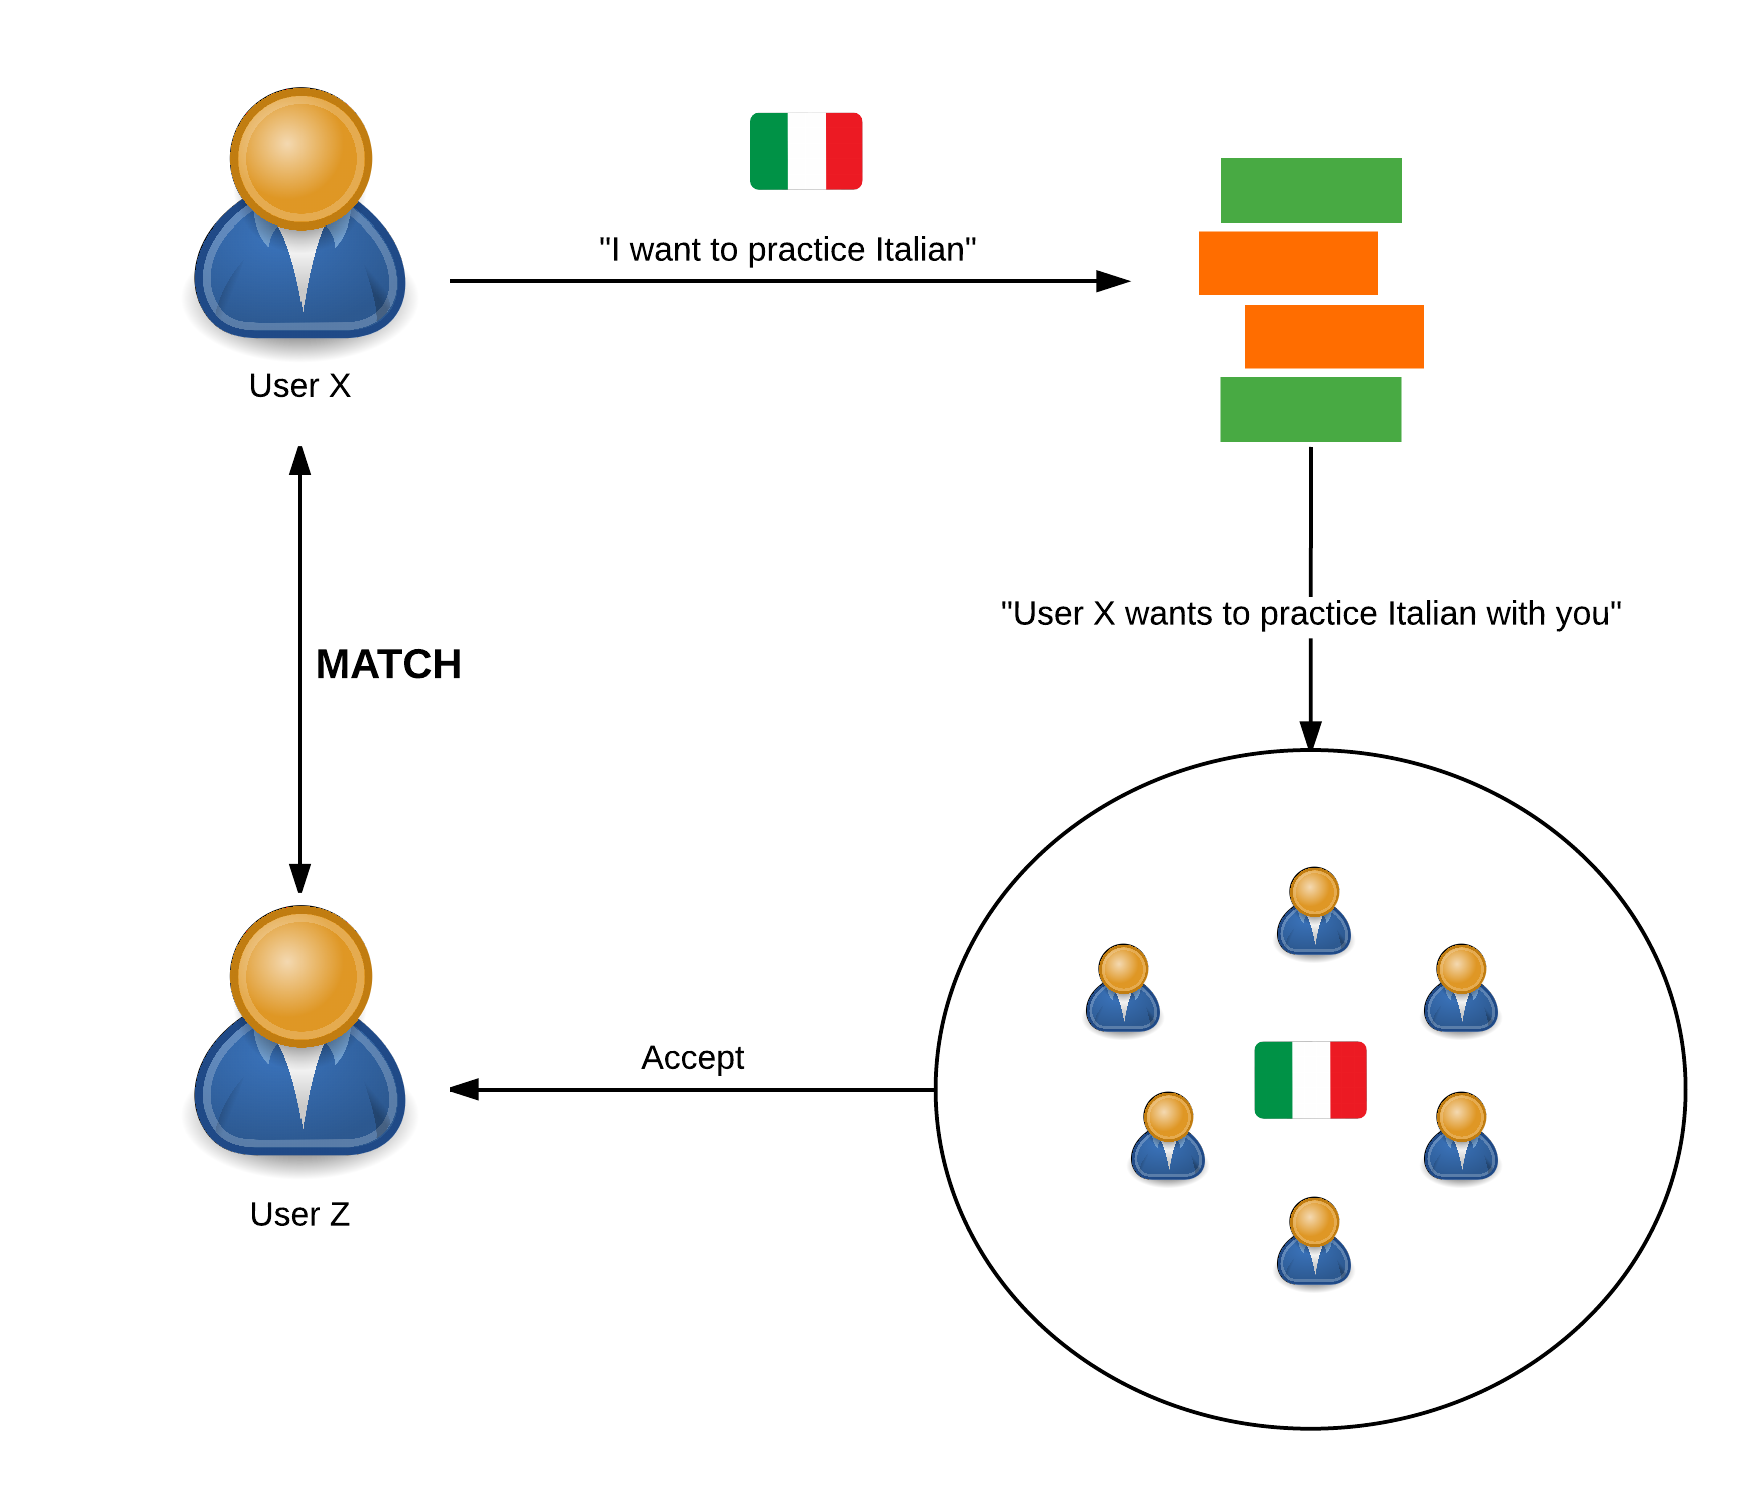
\includegraphics[width=\textwidth]{../immagini/coffeestrap-flow}
\caption{Flusso utente}
\end{figure}

Gli utenti vengono notificati tramite \textbf{notifica email} e, in seguito allo sviluppo dell'applicazione, \textbf{notifica mobile}.

\section{Metodologie e strumenti di sviluppo}

CoffeeStrap adotta la metodologia di sviluppo \textbf{\gls{agile}}. Il particolare contesto entro il quale si trova fa sì che i requisiti cambiano molto spesso e porta dunque quest'ultima a dover iterare molto velocemente sul proprio prodotto, che si trova ancora nella sua fase primordiale e necessita di modifiche e miglioramenti costanti. Proprio a fronte di queste necessità è importante mantenere la massima flessibilità possibile nello sviluppo, motivo per cui questo modello di ciclo di vita è in questo momento il più conveniente in termini di efficienza ed efficacia. In particolare la metodologia adottata è quella \textbf{agile \gls{scrum}}.

Il tipo di iterazione utilizzata è su base settimanale. Una volta a settimana, normalmente il Mercoledì, avviene lo \textbf{scrum meeting}, una riunione della durata di circa due ore nella quale si fissano \textbf{stories} da risolvere nello \textbf{\gls{sprint}} corrente. Una story è un concetto molto simile a quello di \textbf{ticket}, ed è composta dai seguenti campi:

\begin{itemize}

\item \textbf{Titolo};
\item \textbf{Tipologia}, che può assumere i seguenti valori:

	\begin{itemize}

	\item \textbf{Feature}, quando c'è da aggiungere un ``pezzo'' al sistema;
	\item \textbf{Bug}, quando c'è da risolvere una problematica all'interno del sistema;
	\item \textbf{Chore}, quando c'è da eseguire \textit{refactoring} e manutenzione del codice;
	\item \textbf{Release}, sono marcatori di \textit{milestone} che tracciano il progresso del team rispetto agli obiettivi.

	\end{itemize}

\item \textbf{Descrizione}, che fornisce una dettagliata sintesi della story.
\item Una o più \textbf{etichette}, che forniscono un filtro alle stories;
\item \textbf{Complessità}, che è un indice soggettivo di quante risorse sono necessarie per il completamento della story. Questo valore segue la sequenza di Fibonacci e può assumere i valori 1, 2, 5, 8, 13. Se una story ha una complessità superiore a 13 essa dev'essere necessariamente spezzata in due o più sotto-stories. Solamente alle features può essere assegnata complessità, in quanto sono le uniche stories che realmente forniscono un valore al business;
\item \textbf{Richiedente}, che dev'essere unico;
\item Uno o più \textbf{responsabili} (\textit{owners}), che possono coincidere con il richiedente e sono coloro che devono occuparsi direttamente della story;

\end{itemize}

Opzionalmente inoltre è possibile aggiungere alla story dei tasks, in modo da dividere ulteriormente il lavoro. Ciononostante su di essi non vi è alcun controllo, in quanto il loro utilizzo è a discrezione dei responsabili.

\begin{center}
\begin{table}[htpd]
  \begin{tabularx}{\textwidth}{ | c | X |}
    \hline
    \textbf{Titolo} & Login/registrazione con Facebook \\
    \hline
    \textbf{Tipologia} & Feature \\
    \hline
    \textbf{Descrizione} & È necessario interfacciarsi con le API di facebook per Android per poter implementare il sistema di login/registrazione tramite facebook. Una volta ottenuto il token di accesso l'applicazione deve effettuare una chiamata API a CoffeeStrap fornendo quest'ultimo e memorizzando il cookie restituito dalla chiamata. \\
    \hline
    \textbf{Etichette} & \texttt{Mobile} \\
    \hline
    \textbf{Complessità} & 8 \\
    \hline
    \textbf{Richiedente} & Alessandro Maccagnan \\
    \hline
    \textbf{Responsabili} & Luca De Franceschi \\
    \hline
  \end{tabularx}
  \caption{Un esempio di story}
 \end{table}
\end{center}

Ciascuna story è inserita all'interno di una \textbf{board}. Ci sono tre tipologie di board:

\begin{itemize}

\item \textbf{Current}, contenente le stories attive nello sprint corrente;
\item \textbf{Backlog}, contenente la ``coda'' delle stories da attivare;
\item \textbf{Icebox}, contente stories in attesa di approvazione e attivazione. Le stories possono rimanere su questa board per un tempo indeterminato, finché vengono spostate sul backlog o rimosse definitivamente.

\end{itemize} 

A ciascun membro del team vengono assegnate una o più stories, la cui scadenza è lo scrum meeting successivo. A quest'ultimo viene richiesto inoltre di assegnare la complessità a quella story, la quale dovrà essere calcolata secondo criteri derivati dalla propria esperienza di sviluppo. Ogni story dev'essere analizzata, progettata, sviluppata e infine testata. La chiusura della story viene effettuata solamente al seguito di una verifica e validazione da parte del responsabile e del richiedente o, se il richiedente coincide con il responsabile, da un altro membro del team. In generale i responsabili non possono approvare le proprie stories.

Una volta creata la story deve passare attraverso diverse fasi, per questo si parla di \textbf{story workflow}:

\begin{enumerate}

\item La story viene \textbf{creata} e \textbf{definita} (\textit{define and design});
\item I responsabili assegnano loro una \textbf{stima di complessità}, che va generalmente discussa all'interno del team (\textit{estimate});
\item La story viene \textbf{attivata}: da questo momento i responsabili possono procedere allo sviluppo (\textit{start});
\item La story una volta implementata viene \textbf{testata} (\textit{test});
\item Superata la fase di testing la story viene \textbf{ultimata} (\textit{finish});
\item A questo punto i responsabili ``pushano'' il codice sull'ambiente di \textbf{staging} (\textit{deliver});
\item La story viene poi \textbf{accettata} dal richiedente o comunque da una persona esterna al gruppo di responsabili e viene effettuato il pushing sull'ambiente di \textbf{production} (\textit{accept}). Se la story non viene accettata si itera dal punto 4;
\item Infine, se la story è stata accettata avviene il suo \textbf{rilascio}, che coincide con la terminazione del suo ciclo di vita (\textit{release}).

\end{enumerate}

\begin{figure}[htpd]
\centering
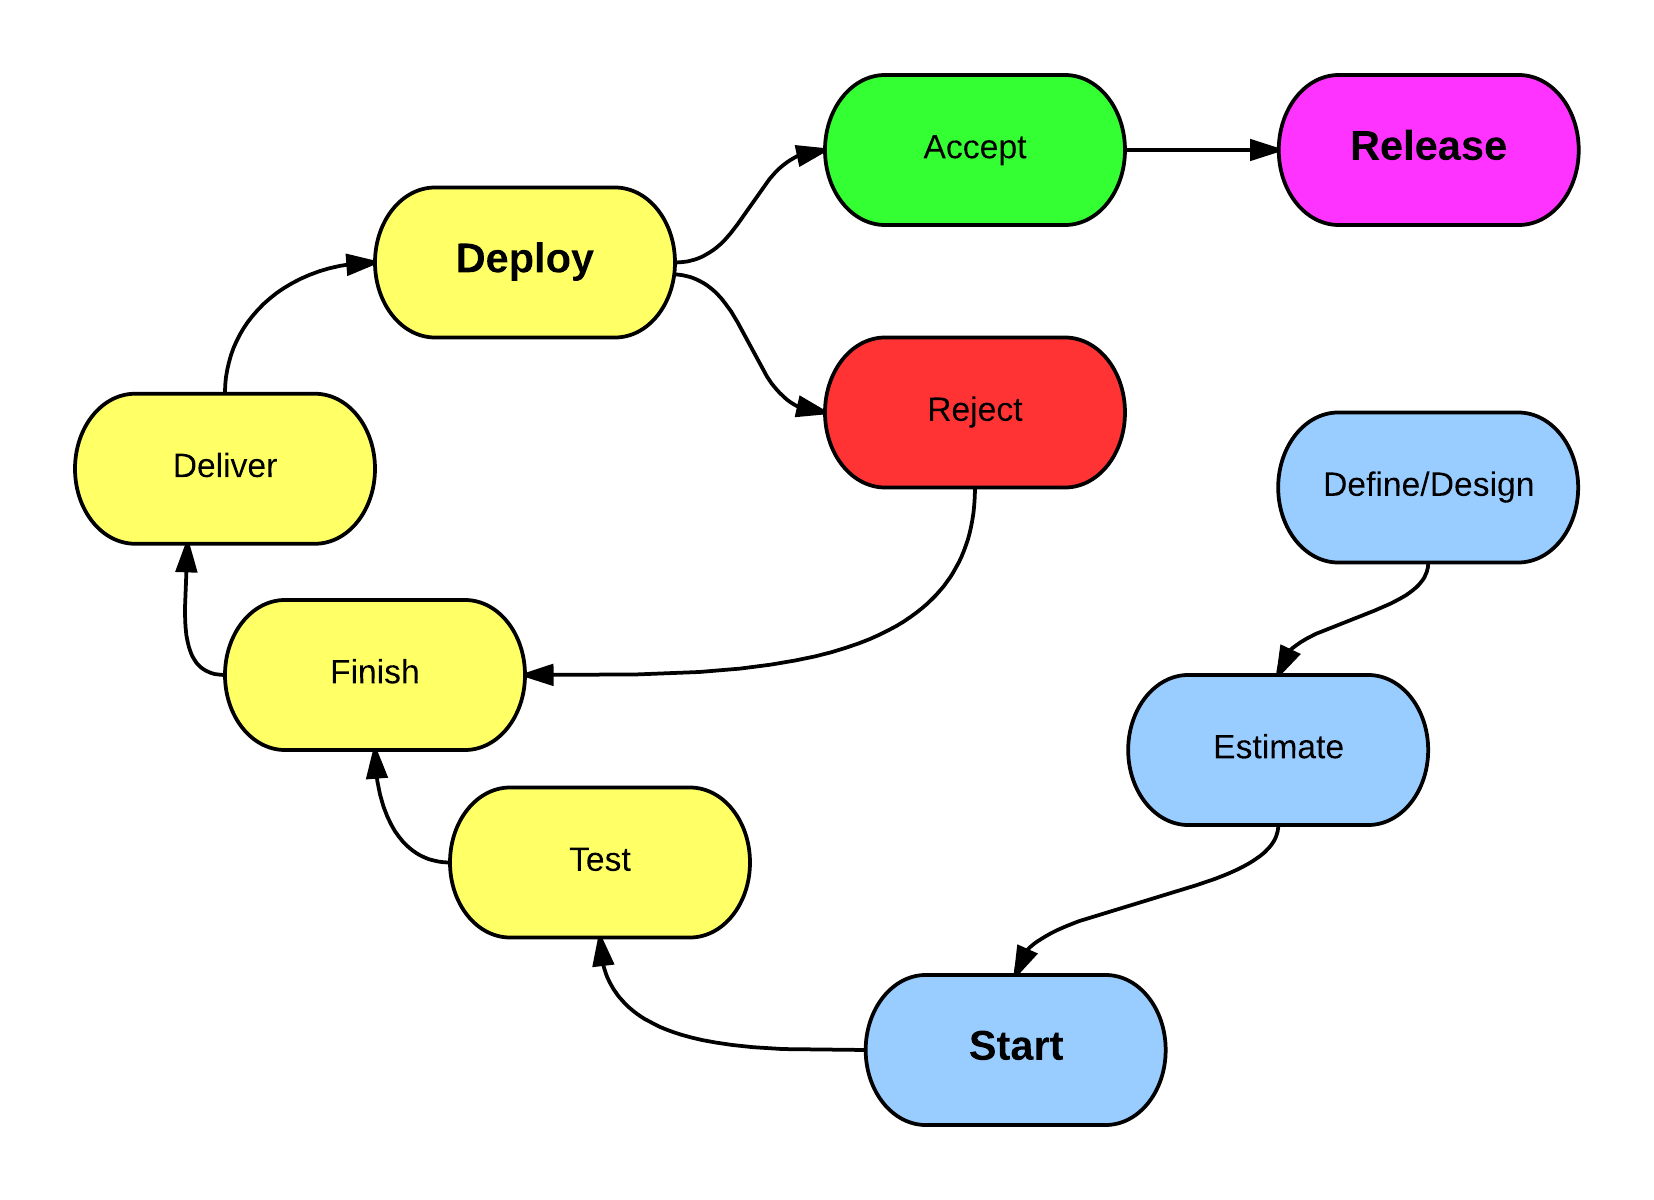
\includegraphics[width=\textwidth]{../immagini/story-workflow}
\caption{Il flusso di una story}
\end{figure}

Alla fine dello sprint viene tracciata la somma delle complessità di tutte le stories assegnate a tutti i membri e che sono state chiuse nello sprint corrente. Tale somma è detta \textbf{velocity}, ed è un indice di efficienza di sviluppo dello sprint, che va confrontato con gli sprint precedenti.

Oltre allo scrum meeting viene instanziato quotidianamente lo \textbf{stand-up meeting}, detto anche \textbf{daily scrum}, nel quale prima dell'inizio della giornata lavorativa si effettua una breve riunione con il team, in cui ciascuno espone quanto fatto nel giorno precedente e ciò che ha in programma di fare nel giorno corrente. Quest'attività è di fondamentale importanza per \textbf{monitorare} il progresso dello sprint e sollevare eventuali difficoltà riscontrate nello svolgimento della story. 

\section{Tecnologie}

\subsection{Back-end}

Il back-end è composto da un server scritto tramite il framework \gls{Node.js}. Questa scelta è dovuta alla grande potenza e scalabilità di quest'ultimo, oltre al fatto che si tratta di un linguaggio di programmazione all'avanguardia la cui comunità è in forte espansione. Inoltre tramite \textbf{npm}, gestore di pacchetti per Node.js, è possibile attingere ad una vasta quantità di librerie.

Il server fornisce tutta una serie completa di \textbf{\gls{API} \gls{REST}ful} accessibili dall'esterno, alcune delle quali richiedono autenticazione. Ciò permette a tutti i client che si interfacciano con esso, in particolare l'applicazione web e l'applicazione mobile, di poter comunicare con esso in modo semplice e lineare, dovendo riferirsi solamente alle specifiche di queste ultime ed utilizzando una libreria per la gestione delle chiamate API. 

\begin{figure}[htpd]
\centering

\includegraphics[width=\textwidth/2]{../immagini/node-js-logo}
\caption{Logo di Node.js}
\end{figure}

Parallelamente al server è stato instanziato un servizio di \textbf{pushing} fornito da \textbf{firebase}, un \textbf{\gls{Cloud Service Provider}} utilizzato per il sistema di notifiche e per fornire un punto d'accesso centralizzato dal quale i diversi componenti (intesi come componenti software) possono comunicare. Firebase fornisce infatti un \textbf{database in tempo reale}, con il quale è possibile interagire e ``\textit{mettersi in ascolto}'' degli eventi su di esso. Esso fornisce un'API pubblica per diversi stack tecnologici e piattaforme.

\begin{figure}[htpd]
\centering

\includegraphics[width=\textwidth/2]{../immagini/firebase-logo}
\caption{Logo di Firebase}
\end{figure}

\subsection{Front-end}

Il front-end è composto da un'applicazione web scritta con \textbf{\gls{Angular.js}} e \textbf{\gls{HTML5}}, utilizzando il framework CSS \textbf{\gls{Bootstrap}}. Tramite Angular.js è possibile interfacciarsi alle API fornite dal back-end in maniera molto efficiente e popolare dunque le pagine in base alle risposte provenienti da esso. Inoltre, analogamente a npm, per lo sviluppo di applicazioni con Angular.js è disponibile \textbf{bower}, gestore di pacchetti per quest'ultimo.

\begin{figure}[htpd]
\centering

\includegraphics[width=\textwidth/2]{../immagini/angular-js-logo}
\caption{Logo di Angular.js}
\end{figure}

\subsection{Database}

CoffeeStrap utilizza \textbf{\gls{MongoDB}} come database documentale di riferimento. Questa scelta è dovuta alla grande flessibilità offerta dai database di questo tipo, oltre al fatto che negli ultimi mesi è divenuto molto popolare nella comunità di sviluppatori e presenta prestazioni notevoli. 

Dal momento che i requisiti cambiano molto rapidamente è necessario avvalersi di strumenti che siano il più flessibili possibili ai cambiamenti, e MongoDB risponde perfettamente a questo tipo di esigenza. Inoltre MongoDB presenta un facile approccio al suo utilizzo sia per l'utilizzo da parte dello sviluppatore che in termini di scalabilità.

\begin{figure}[htpd]
\centering

\includegraphics[width=\textwidth/2]{../immagini/mongo-db-logo}
\caption{Logo di MongoDB}
\end{figure}

\subsection{Ambienti di sviluppo}

All'interno dell'azienda si delineano principalmente due ambienti di sviluppo:

\begin{itemize}

\item \textbf{Production}, all'interno del quale risiedono le versioni ufficiali del codice esposte pubblicamente agli utenti;

\item \textbf{Staging}, un ambiente riservato esclusivamente al team e che rappresenta una sorta di ``cantiere'', nel quale risiede una versione del codice ancora da verificare, che può quindi essere testata liberamente e non crea danni verso l'esterno.

\end{itemize}

Ciascun ambiente è caratterizzato dalla propria configurazione, possiede il proprio server e il proprio database ed è agnostico rispetto all'altro.

Occasionalmente è inoltre uso comune instanziare un ambiente ausiliario di sviluppo, per circostanze particolari che necessitano di una configurazione diversa. Solitamente sono ambienti ``\textit{usa e getta}'', che nascono da esigenze particolare e vengono rimossi alla fine del loro utilizzo.

\subsection{Versionamento}

Come strumento di controllo versione del codice sorgente l'azienda utilizza \textbf{\gls{Git}}, utilizzando \textbf{Bitbucket} come servizio di hosting. I motivi che hanno spinto all'utilizzo di Git in luogo di altri sistemi di versionamento sono i seguenti:

\begin{itemize}

\item \textbf{Disponibilità}: ciascun sviluppatore ha una copia locale dell'intero repository ed effettua \textit{\gls{commit}} in locale, potendo dunque lavorare anche in assenza di connessione;

\item \textbf{Semplicità}: oltre ad essere veloce Git permette con facilità la creazione di \textit{branch} e successivi \textit{\gls{merge}}. L'utilizzo di questi ultimi è fondamentale per poter soddisfare il punto seguente:

\item \textbf{Utilizzo di Gitflow}: questo \textbf{workflow} definisce uno stretto modello di \textit{branching} che ruota intorno al progetto. Ciò non aggiunge nuovi concetti o strumenti a Git, ma piuttosto assegna ruoli specifici ai diversi rami. Un approfondimento di questa metodologia è raccolta nell'appendice A.

\end{itemize}

\begin{figure}[htpd]
\centering

\includegraphics[width=\textwidth/2]{../immagini/git-logo}
\caption{Logo di Git}
\end{figure}

\section{Clientela di riferimento}

CoffeeStrap non ha ancora acquisito finanziamenti da parte di investitori e non presenta associazioni con altre aziende o entità, motivo per cui essi devono rispondere unicamente agli \textbf{utenti finali} del prodotto. Questi ultimi sono persone reali provenienti da ogni parte del mondo, che mettono a disposizione le proprie competenze linguistiche e vogliono allo stesso tempo imparare una lingua straniera entrando in contatto con altri utenti. L'intera struttura di CoffeeStrap si basa su questa \textbf{rete sociale}, composta da un insieme eterogeneo di persone che espongono il proprio profilo all'esterno. È possibile immaginare CoffeeStrap come un vero e proprio \textit{social network} il cui scopo è l'apprendimento linguistico.

\begin{figure}[htpd]
\centering
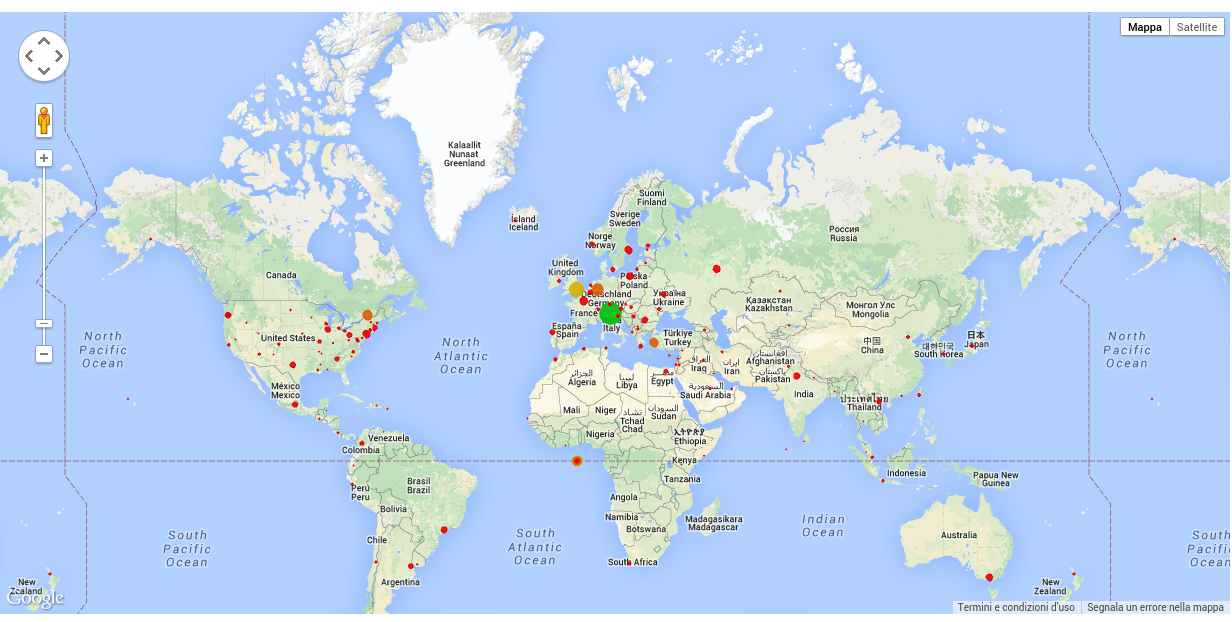
\includegraphics[width=\textwidth]{../immagini/user-distribution}
\caption{Distribuzione degli utenti di CoffeeStrap nel mondo aggiornata a Dicembre 2014}
\end{figure}           
% !TEX encoding = UTF-8
% !TEX TS-program = pdflatex
% !TEX root = ../tesi.tex
% !TEX spellcheck = it-IT

%**************************************************************
\chapter{Il progetto all'interno dell'azienda}
\label{cap:progetto-azienda}
%**************************************************************

\section{Presentazione del progetto}

Il progetto svolto da me durante l'attività di stage consiste nello sviluppo di un'applicazione mobile, sviluppata nativamente in Android, che replica il meccanismo e il flusso utente già esistente nel web integrandolo all'interno di questo tipo di piattaforma. 

\subsection{Motivazioni}

Come già presentato nel capitolo 1, CoffeeStrap ha come primo e unico scopo lo sviluppo di una piattaforma peer-to-peer per l'appredimento di una lingua tramite interazioni tra utenti. Lo scopo principale in questa prima fase di sviluppo è quella di raccogliere un bacino utenti considerevole, in modo da poter capire su quale linea portare avanti l'idea e modellare quest'ultima in base al \textit{feedback} e al tipo di iterazione dell'utente medio. Prima dell'inizio del mio stage CoffeeStrap disponeva solamente dell'applicazione web, la quale possedeva circa 2000 iscritti e mediamente 15 utenti attivi al giorno. 

Il progetto di stage che ho svolto nasce dunque dalla necessità di affiancare all'applicazione web l'applicazione mobile, in modo da poter fornire all'utente più possibilità di utilizzo del prodotto ed arrivare inoltre ad un considerevole incremento del bacino utenti. La considerazione pricipale a monte di ciò è il fatto che oggigiorno l'utente medio spende la maggior parte del proprio tempo sul proprio smartphone piuttosto che sul proprio pc, per tutti i vantaggi legati alla tecnologia mobile. È di fatto una necessità imprescindibile per una start-up in ambito \textit{web/mobile} estendersi su più piattaforme se si vuole competere in un certo tipo di mercato ed ottenere dei finanziamenti. In aggiunta CoffeeStrap può essere categorizzato di fatto come \textit{social newtwork}, ulteriore motivo per il quale sviluppare il prodotto su mobile è di importanza fondamentale.

L'avere a disposizione l'applicazione a qualsiasi ora del giorno e in qualsiasi luogo permette all'utente di fruire del prodotto senza limitazioni e nel momento esatto in cui ne sente la necessità. Da questo ne deriva un aumento del numero di iterazioni e della quantità di utenti attivi giornalieri, dati di fondamentale importanza per gli investitori.

Possiamo sintetizzare in otto punti i vantaggi per cui un'azienda dovrebbe avere un'applicazione mobile:

\begin{enumerate}

\item \textbf{Visibilità}: i dati rilevati indicano che le ricerche all'interno degli \textit{App stores} siano molto elevate, motivo per cui comparire tra i risultati di ricerca rappresenta un'ottima \textbf{pubblicità} per l'azienda;
\item \textbf{Aumento del valore del brand}: avere la propria applicazione è indice di un'azienda \textit{dinamica}, sempre attenta all'evoluzione tecnologica e al passo coi tempi. Questi valori aumentano di molto il valore dell'azienda;
\item \textbf{Copertura mediatica}: con la tecnologia mobile è possibile coprire anche zone con scarsa connettività ad internet, coprendo una zona molto maggiore ed aprendo nuove possibilità per il business;
\item \textbf{Crescita del mercato mobile}: il mondo mobile è in grossa crescita e prospera più velocemente rispetto al web. Lo smartphone è al giorno d'oggi uno strumento essenziale per qualsiasi persona, sia per il tempo libero che per il lavoro.
\item \textbf{Capacità di differenziarsi dai concorrenti}: le aziende concorrenti che non dispongono di un'applicazione mobile passano in secondo piano rispetto ad un'azienda che ne dispone.

\end{enumerate}

\subsection{Aspettative}

La mia preparazione e formazione in ambito di sviluppo mobile poteva ritenersi pari a zero all'inizio dell'attività di stage. Cionostante l'azienda era consapevole di quali fossero le mie capacità, avendo già collaborato con me e il mio \textit{team} per il progetto di ingegneria del software dell'anno accademico 2013/2014. Pochi mesi prima, in collaborazione con il team \textbf{steakholders}, avevo infatti sviluppato un framework per l'amministrazione di dati provenienti da MongoDB. CoffeeStrap ha assunto il ruolo di \textbf{committente} all'interno di questo progetto, quindi vi erano state diverse interazioni tra me e l'azienda, la quale tuttora utilizza quotidianamente come strumento di supporto.

A fronte della realizzazione di questo progetto l'azienda poneva in me delle buone aspettative circa le tempistiche di apprendimento della tecnologia e di integrazione all'interno del team, per cui il \textbf{rischio} di ospitare un'attività di stage era mitigato da questi fattori. Inoltre i membri di CoffeeStrap, avendo frequentato anch'essi il mio stesso corso di studi, erano al corrente di quale tipo di formazione l'università di Padova offrisse agli studenti e in particolare in che modo e secondo quali prassi il corso di \textit{Ingegneria del Software} preparasse questi ultimi ad essere inseriti velocemente nel mondo del lavoro, avendo alle spalle un'esperienza corposa ed istruttiva. Queste motivazioni hanno fatto sì che l'azienda decidesse di ospitare al loro interno un'attività di stage che potesse soddisfare gli obiettivi preposti. 

Considerando la durata dello stage e le tempistiche legate all'apprendimento della tecnologia, l'aspettativa da parte dell'azienda era quella di arrivare alla fine del periodo di stage con in mano un \textbf{prototipo funzionante}, pronto per essere inserito in una fase successiva di test più approfondito e di raffinamento dei componenti, comunque non ancora sufficientemente maturo per essere inserito pubblicamente nel mercato. L'aspettativa era quella di una versione dell'applicazione che in ambito informatico viene generalmente indicata come \textit{beta}.

Gli obiettivi minimi delineati sono i seguenti:

\begin{itemize}

\item \textit{Signup} e \textit{login} all'applicazione da parte dell'utente;
\item Visualizzazione e modifica delle preferenze da parte dell'utente;
\item Comunicazione audio;
\item Sistema di notifica, quest'ultimo punto fondamentale all'interno del progetto;

\end{itemize}

Oltre agli obiettivi minimi inoltre sono stati posti degli obiettivi massimi:

\begin{itemize}

\item Comunicazione testuale;
\item Comunicazione video;

\end{itemize}

Durante il corso dell'attività di stage ciononostante i requisiti sono aumentati, in base alla necessità di realizzare appieno il flusso previsto, il quale è stato riprogettato nel medesimo periodo. Gli obiettivi sono dunque rimasti invariati ma sono stati aggiunti i seguenti:

\begin{itemize}

\item Richiesta di un \textbf{match} in base a una lingua, dove per \textit{match} si intende un \textit{collegamento} tra due utenti mantenibile nel tempo;
\item Notifica di invito da parte di un utente di parlare una lingua;
\item Creazione e mantenimento della lista di match;

\end{itemize}

Questi ultimi sono stati necessari per arrivare ad un'applicazione con un grado di usabilità accettabile.

\subsection{Obiettivi di formazione}

L'azienda, essendo di piccole dimensioni e in fase primordiale, ha come prima necessità, oltre allo sviluppo e diffusione del prodotto, la formazione di un team qualificato con all'interno elementi di natura tecnica.  Nelle aziende di questo tipo la prima necessità e risorsa sono le \textbf{persone}, in quanto il valore dell'azienda deriva dal lavoro dei suoi dipendenti. A fronte di questa necessità ospitare un'attività di stage permette all'azienda di poter integrare personale giovane, con una buona formazione e dotati di forte motivazione e stimoli, oltre che una buona elasticità mentale. 

Tra gli obiettivi formativi si delineano i seguenti:

\begin{itemize}

\item Apprendimento della tecnologia mobile, in particolare introduzione all'utilizzo della piattaforma Android;
\item Apprendimento del protocollo REST e comunicazione lato server tramite API;
\item Formazione sullo sviluppo di servizi di terze parti utilizzate dall'azienda; 
\item Introduzione alla metodologia agile scrum;
\item Introduzione al contesto della start-up e alla sua particolare realtà.

\end{itemize}

\section{Vincoli}

\subsection{Vincoli tecnologici}

All'inizio dello stage è stata fatta una valutazione riguardo lo \textit{stack tecnologico} da adottare per la realizzazione dell'applicazione. Sono state delineate tre possibilità:

\begin{itemize}

\item \textbf{Titanium}\footnote{\url{http://www.appcelerator.com/titanium/}}, un framework di sviluppo mobile basato su \textit{javascript} e \textit{HTML5}, che permette lo sviluppo su più piattaforme;

\item \textbf{Ionic}\footnote{\url{http://ionicframework.com/}}, altro framework ibrido molto simile al precedente;

\item \textbf{Nativo Android}, in cui viene messo a disposizione un vero e proprio SDK ufficiale per lo sviluppo, basato su Java.

\end{itemize}

Il vantaggio delle prime due è quello legato all'utilizzo di questo genere di framework, ovvero la possibilità di effettuare un \textit{delivery} rapido e multipiattaforma di un'applicazione. Il codice, infatti, si scrive velocemente con un meta linguaggio ed attraverso librerie esterne precompilate esso viene adattato per i diversi sistemi operativi in fase di compilazione. 

D'altra parte una \textbf{criticità} di questi framework consiste nella loro rigidità in fase progettuale: il loro utilizzo, infatti, limita in parte la possibilità di sfruttare le caratteristiche native del \textit{device}, delle linee guida dell'interfaccia e del sistema operativo su cui avverrà il \textit{deploy} dell'applicazione. Spesso dunque si corre il rischio di non arrivare ad un prodotto conforme alle attese con un'interfaccia utente poco ergonomica e intuitiva. Inoltre non è garantito un supporto su lungo periodo alle medesime condizioni. Alcuni framework tendono infatti a non essere più supportati dopo un lungo periodo e il rischio è quello di dover riprogettare tutto daccapo.

Sviluppare un'applicazione nativa garantisce quindi maggiore efficienza in fase di sviluppo e progettazione e porta ad un risultato migliore in termini di usabilità. Chiaramente lo svantaggio è quello di poter supportare un solo sistema operativo, motivo per cui in un futuro CoffeeStrap dovrà ad esempio instanziare un nuovo progetto per l'applicazione \textit{iOS}, molto richiesta dal mercato.

Alla fine la scelta è ricaduta proprio sullo sviluppo nativo, quindi il vincolo tecnologico principale è stato lo sviluppo su piattaforma Android, utilizzando l'SDK ufficiale, ovvero il vero e proprio pacchetto di strumenti che permette lo sviluppo su questa piattaforma. Esso viene normalmente scaricato all'interno di ambienti di sviluppo integrati (IDE), in particolare \textit{Eclipse} e \textit{Android Studio}. Non è stato posto un vincolo circa la scelta di quest ultimo, che è stata totalmente a carico mio. Questi ambienti mettono a disposizione, oltre ad un ambiente di programmazione, anche strumenti per il design delle diverse schermate, che viene realizzato utilizzando il linguaggio \textit{XML}. 

È stata inoltre richiesta l'integrazione all'interno dell'applicazione di tutti i servizi utilizzati dall'azienda per i diversi requisiti:

\begin{itemize}

\item Utilizzo dell'\textbf{SDK di facebook} per il login e signup all'applicazione da parte dell'utente;
\item Utilizzo della libreria di \textbf{firebase} per il sistema di \textit{pushing};
\item Utilizzo di una libreria per la gestione delle chiamate API al server, la quale è stata scelta e discussa durante la fase di progettazione;
\item Utilizzo della libreria \textbf{bugsnag}, per il servizio di \textit{bug tracking};
\item Utilizzo della libreria \textbf{opentok} per il servizio di comunicazione audio/video;
\item Utilizzo della libreria di \textbf{mixpanel} per il servizio di \textit{web/mobile analysis}.

\end{itemize} 

\subsection{Vincoli metodologici}

CoffeeStrap ha ritenuto importante il mio inserimento all'interno del team e l'apprendimento da parte mia delle loro metodologie di lavoro, pertanto fin dalla prima settimana sono stato inserito all'interno dei meccanismi di sviluppo agile, ho partecipato attivamente agli scrum meeting e agli stand-up meeting e ho creato e svolto le mie stories con gli stessi procedimenti attuati dagli altri membri. 

Oltre a questo c'è stato un monitoraggio costante da parte del \textit{tutor} aziendale sui processi e le metodologie da me instanziati per l'apprendimento e lo sviluppo della tecnologia, che hanno fatto sì che prendessi gradualmente confidenza con il \textit{modus operandi} adottato dall'azienda.

\subsection{Vincoli temporali}

Lo stage viene distribuito in 8 settimane di calendario, per una durata complessiva di 300-320 ore lavorative. Ogni settimana sono previste 40 ore, considerando una giornata lavorativa composta di 8 ore. Lo stage può dunque considerarsi un'attività a tempo pieno.

Nonostante questo vincolo temporale imposto le modalità operative non prevedevano un conteggio delle ore lavorative, ma erano basate sullo svolgimento delle \textit{stories}, descritte nel capitolo 1. A fronte di ciò posso affermare che quanto realizzato a livello di ore lavorative differisce in eccesso rispetto a quanto pianificato, in quanto la completa libertà di gestire il proprio tempo ha fatto sì che molto spesso le mie giornate lavorative si prolungassero oltre le 8 ore e che il sabato e la domenica (giorni non considerati in un calendario lavorativo) venissero frequentemente spesi nello sviluppo dell'applicazione.

In nessun modo CoffeeStrap ha imposto vincoli temporali superiori a quanto pattuito. Queste scelte da me effettuate sono state puramente personali, derivate dalla forte motivazione e sollecitazione date dal progetto, di per sè molto stimolante, e dalla crescente voglia di imparare.             
% !TEX encoding = UTF-8
% !TEX TS-program = pdflatex
% !TEX root = ../tesi.tex
% !TEX spellcheck = it-IT

%**************************************************************
\chapter{Il progetto di stage}
\label{cap:descrizione-stage}
%**************************************************************

\section{Pianificazione del lavoro}

In questa sezione descriverò come il progetto è stato suddiviso nell'arco delle otto settimane e quali erano gli obiettivi alla fine di ciascun periodo.

\section{Norme, procedure e strumenti}

In questa sezione descriverò tutte le norme e le procedure con il quale ho organizzato il mio lavoro, quali processi ho attuato con le loro motivazioni e di quali strumenti mi sono avvalso per l'attuazione di tali processi.

\section{Periodo di formazione}

\subsection{Apprendimento della tecnologia}

In questa sezione descriverò come ho appreso la tecnologia di riferimento e attraverso quali processi, approfondendo nel dettaglio alcuni concetti indispensabili e di rilievo. Descriverò la differenza tra le mie conoscenze alla fine di questo periodo e all'inizio, fornendo evidenza di apprendimento.

\subsection{Integrazione con le tecnologie aziendali}

In questa sezione descriverò come, dopo uno studio della tecnologia legata al progetto di stage abbia integrato quest'ultima con le tecnologie già esistenti utilizzate all'interno dell'azienda.

\section{Progettazione}

\subsection{Progettazione del flusso utente}

In questa sezione descriverò la progettazione del flusso utente all'interno dell'applicazione Android, avvalendomi di diagrammi di attività e di flusso.

\subsection{Progettazione del layout}

In questa sezione descriverò la progettazione del layout delle diverse schermate dell'applicazione, giustificando le varie scelte secondo criteri di accessibilità e usabilità.

\subsection{Progettazione architetturale}

In questa sezione descriverò la progettazione dell'architettura software dell'applicazione, andando ad evidenziare la suddivisione in classi e pacchetti, le interazioni di quest'ultimi, le librerie esterne e i design pattern utilizzati; il tutto in relazione con le best-practise indicate dalla comunitò di sviluppatori Android.

\section{Sviluppo e codifica}

In questa sezione descriverò come ho realizzato il codice dell'applicazione aderendo alla progettazione attuata in precedenza.

\section{Rifinitura e testing}

In questa sezione descriverò come a fronte dello sviluppo e codifica dell'applicazione ho proceduto alla sua verifica, istanziando un sistema di bug tracking e testando l'applicazione con utenti reali.

\section{Validazione del prodotto e rilascio}

In questa sezione infine descriverò come a fronte dell'attività di rifinitura è stata istanziata un'attività di validazione mirata a verificare che il prodotto corrispondesse alle aspettative e soddisfasse gli obiettivi preposti. Inoltre descriverò l'attività di rilascio e di pubblicazione di una versione sul play store di Google.             
% !TEX encoding = UTF-8
% !TEX TS-program = pdflatex
% !TEX root = ../tesi.tex
% !TEX spellcheck = it-IT

%**************************************************************
\chapter{Valutazioni retrospettive}
\label{cap:analisi-requisiti}
%**************************************************************

\section{Bilancio sui risultati}

In questa sezione darò evidenza di aver soddisfatto tutti gli obiettivi di stage, fornendo un consuntivo di quanto realizzato, confrontato con il preventivo di inizio stage.

\section{Bilancio formativo}

In questa sezione confronterò la mia formazione all'inizio dello stage con quella ottenuta alla fine, evidenziando quanto appreso e il tipo di maturazione ottenuta sul piano tecnico e metodologico.

\section{Distanza tra contesto lavorativo e mondo accademico}

In questa sezione fornirò un GAP di conoscenze, evidenziando gli elementi nulli sul quale il corso di laurea non è riuscito a formarmi. Fornirò dunque una critica costruttiva nei confronti del mondo accademico, confrontando il mio bagaglio in ingresso con quello in uscita e presentando dei suggerimenti in ottica di miglioramento del corso di laurea.
             

\appendix                               

\chapter{Gitflow}

Gitflow è un modello di sviluppo basato su Git, ideato da Vincent Driessen e presentato nel 2010 in un suo celebre post.\footnote{\url{http://nvie.com/posts/a-successful-git-branching-model/}}. Sebbene sia pittosto complicato rispetto ad altri modelli, questo framework fornisce un robusto strumento per la gestione di progetti di grandi dimensioni.

Gitflow assegna ruoli specifici ai diversi branch, specificando quando e come essi debbano interagire tra di loro. Essendo basato su Git gli sviluppatori lavorano in locale e periodicamente effettuano \textit{push} sul repository remoto centrale.

\section{I branch principali}

Nel repository principale si distinguono due rami principali:

\begin{itemize}

\item \textbf{master}, il ramo principale all'interno del quale risiede codice verificato e pronto per essere spedito in \textit{production} e in particolare tutti i suoi nodi corrispondono a \textbf{release} del prodotto, ovvero ad una versione stabile, che può essere marcata o meno con un \textit{tag};

\item \textbf{develop}, il ramo all'interno del quale avviene lo sviluppo vero e proprio del prodotto e dal quale il codice può essere rilasciato, effettuando dunque un \textit{merge} con il ramo master

\end{itemize}

\section{I branch di supporto}

Al livello inferiore dei branch principali troviamo i branch di supporto, che assistono gli sviluppatori nelle operazioni quotidiane di sviluppo. Questi branch, a differenza dei due principali, hanno un tempo di vita limitato e vengono uniti nei rami principali o semplicemente scartati. I tre branch di supporto sono:

\begin{itemize}

\item \textbf{Feature}, che viene creato dal ramo \texttt{develop} ed unito solamente nel medesimo; la loro utilità, come dice la parola stessa, è quella di creare un ramo di sviluppo per un nuovo componente del sistema. Essi normalmente vanno tenuti in locale e non devono essere \textit{pushati} sul repository remoto;

\item \textbf{Release}, che viene creato dal ramo \texttt{develop} ed unito sia nel medesimo che successivamente su \texttt{master}. Questo branch identifica le procedure che vengono istanziate all'atto della release. Quando uno sviluppatore decide di effettuare una release del prodotto apre innanzitutto un brach da \texttt{develop} chiamato \texttt{release-*}, esegue tutte le operazioni di \textit{pre-release}, effettua il merge su \texttt{develop} ed infine il merge su \texttt{master}, marcando il nodo di merge eventualmente con un \textit{tag};

\item \textbf{Hotfix}, che viene creato dal ramo \texttt{master} ed unito prima sia nel medesimo che successivamente su \texttt{develop}. Questi rami derivano dall'immediata necessità di risolvere un \textit{bug} inserito all'interno del ramo master, senza dover effettuare una nuova release. 

\end{itemize}

\begin{figure}[htpd]
\centering
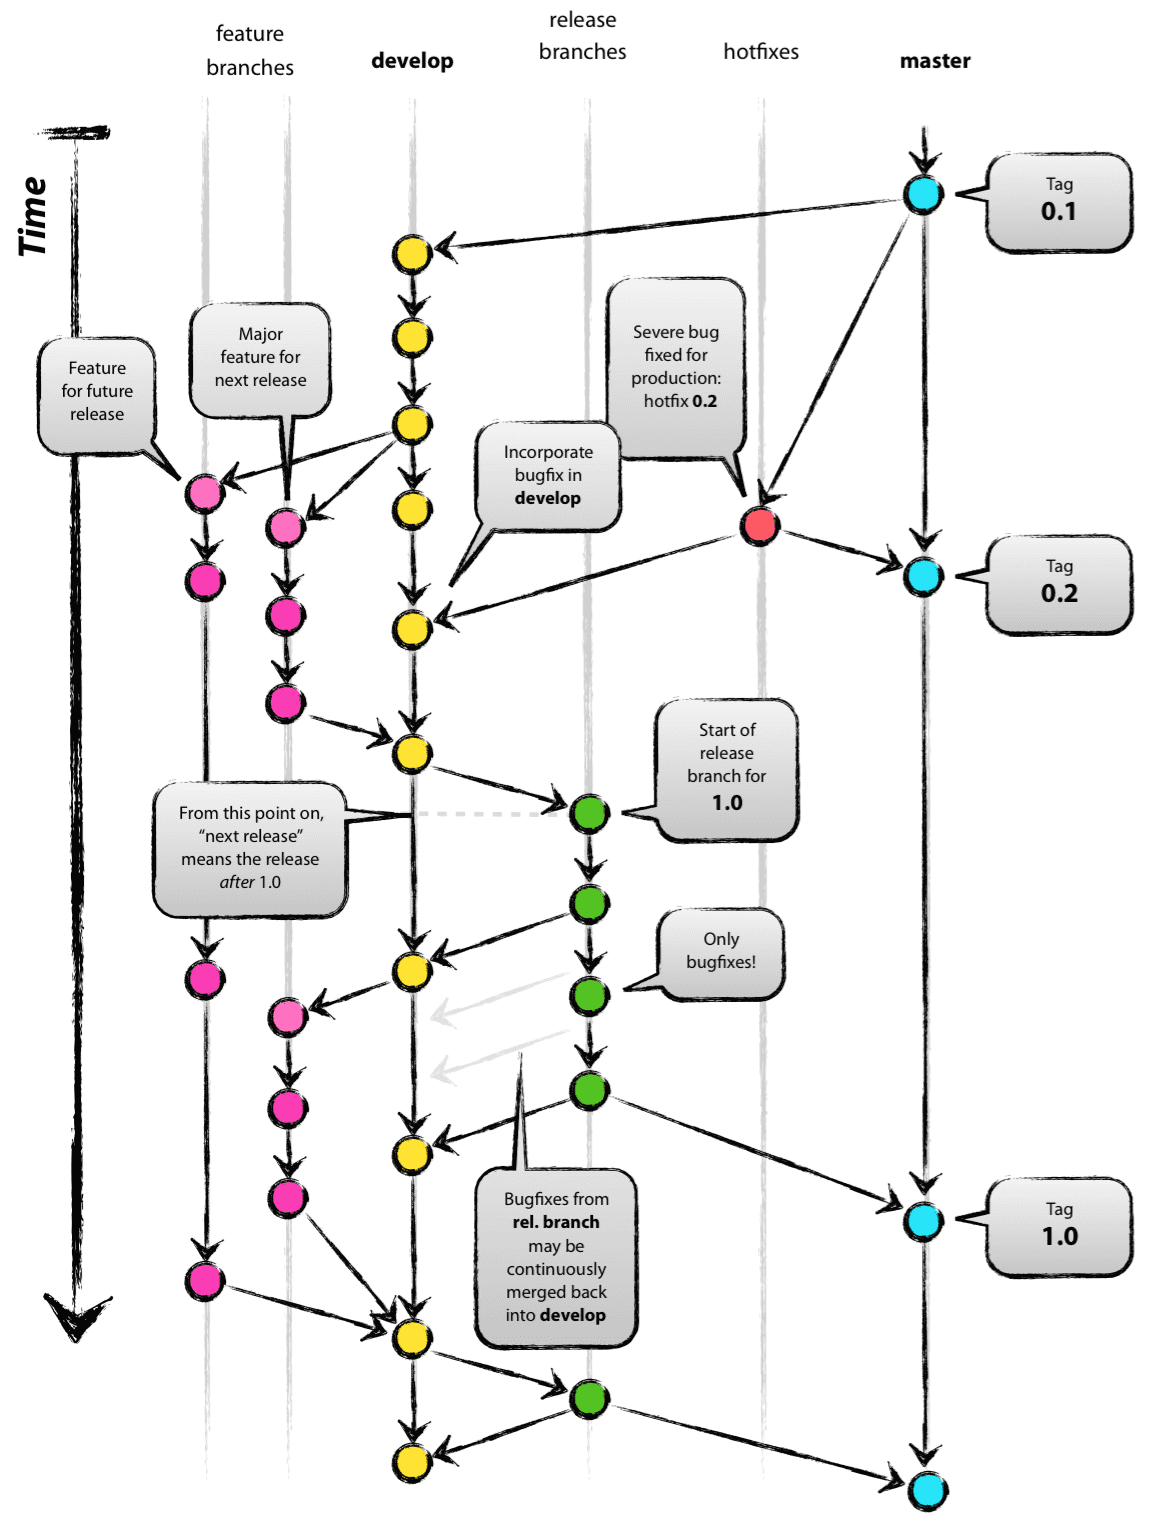
\includegraphics[width=\textwidth/2]{../immagini/git-flow-model}
\caption{Modello Gitflow}
\end{figure}


             % Appendice A

%**************************************************************
% Materiale finale
%**************************************************************
\backmatter
\printglossaries
% !TEX encoding = UTF-8
% !TEX TS-program = pdflatex
% !TEX root = ../tesi.tex
% !TEX spellcheck = it-IT

%**************************************************************
% Bibliografia
%**************************************************************

\nocite{*}
\printbibliography

\bibbycategory % equivale a dare un \printbibliography per ogni categoria


\end{document}